\chapter{Results}
\section{Single-objective optimization}
In this study, the performance of four models, VAE, $\beta$-VAE, CVAE, and $\beta$-CVAE, was evaluated based on the target properties and multi-objective optimization. We recall that all models were trained using the same data set. While the VAE and $\beta$-VAE models generated molecules without any constraints, the CVAE and $\beta$-CVAE models generated molecules under two different conditions defined in (6). Fig. 7 shows a random sample of generated molecules from the models. The performance of the models was evaluated by checking the number of generated molecules that satisfied the target properties within a certain range when provided with conditions within that range. To further confirm the performance of CVAE and $\beta$-CVAE, the number of molecules generated by VAE and $\beta$-VAE that matched the range of each condition was also counted.

The following results were tabulated after validity, novelty, and uniqueness checks: 1) Table 2 shows the percentage of molecular properties within the aforementioned acceptable range; 2) Table 3 shows the descriptive statistical molecular property results of all models presented in this study; 3) Table 4 shows the percentage scores for single-objective and multi-objective property optimization for all models. The non-conditional models (VAE and $\beta$-VAE) were set to generate 10,000 molecules while the conditional models (CVAE and $\beta$-CVAE) were set to generate 10,000 molecules for each condition. The VAE and $\beta$-VAE models generated 17.000\% and 16.300\% of molecules, respectively. The CVAE and $\beta$-CVAE generated 13.316\% and 12.599\% of molecules, respectively. The low percentages of generated molecules suggest that the majority of molecules generated by the models were invalid, not novel, and not unique. 

\begin{table}[htbp]
\caption{Molecular properties within range}
\centering
\resizebox{\columnwidth}{!}{%
\begin{tabular}{|cccc|cccc|}
\hline
\multicolumn{4}{|c|}{\textbf{ClogP (\%)}} & \multicolumn{4}{c|}{\textbf{CMR (\%)}} \\ \hline
\textbf{VAE} & \textbf{$\beta$-VAE} & \textbf{CVAE} & \textbf{$\beta$-CVAE} & \textbf{VAE} & \textbf{$\beta$-VAE} & \textbf{CVAE} & \textbf{$\beta$-CVAE} \\
96.588 & 95.951 & 98.306 & 97.605 & 100.000 & 100.000 & 99.777 & 98.313 \\ \hline
\end{tabular}%
}
\end{table}

\begin{table*}[t]
\caption{Generated Molecular Results}
\resizebox{\textwidth}{!}{%

\begin{tabular}{c|cccc|cccc|cccc|}
\cline{2-13}
 & \multicolumn{4}{c|}{\textbf{CLogP}} & \multicolumn{4}{c|}{\textbf{CMR}} & \multicolumn{4}{c|}{\textbf{Length}} \\ \cline{2-13} 
 & \textbf{VAE} & \textbf{$\beta$-VAE} & \textbf{CVAE} & \textbf{$\beta$-CVAE} & \textbf{VAE} & \textbf{$\beta$-VAE} & \textbf{CVAE} & \textbf{$\beta$-CVAE} & \textbf{VAE} & \textbf{$\beta$-VAE} & \textbf{CVAE} & \textbf{$\beta$-CVAE} \\ \cline{2-13} 
\textbf{mean} & 3.465 & 3.400 & 2.549 & 1.972 & 69.179 & 68.762 & 64.048 & 62.613 & 16.245 & 16.189 & 15.774 & 15.661 \\
\textbf{std} & 1.147 & 1.154 & 1.241 & 1.209 & 5.575 & 5.611 & 7.520 & 8.000 & 1.053 & 1.052 & 1.394 & 1.632 \\
\textbf{min} & -0.119 & -0.698 & -2.527 & -3.463 & 42.272 & 45.787 & 28.779 & 23.419 & 9.000 & 13.000 & 9.000 & 6.000 \\
\textbf{25\%} & 2.688 & 2.662 & 1.702 & 1.180 & 65.694 & 64.920 & 58.797 & 58.083 & 16.000 & 16.000 & 15.000 & 15.000 \\
\textbf{50\%} & 3.446 & 3.323 & 2.520 & 1.980 & 69.523 & 68.731 & 64.614 & 63.683 & 16.000 & 16.000 & 16.000 & 16.000 \\
\textbf{75\%} & 4.199 & 4.106 & 3.359 & 2.776 & 72.893 & 72.828 & 69.616 & 68.274 & 17.000 & 17.000 & 17.000 & 17.000 \\
\textbf{max} & 7.124 & 6.900 & 7.268 & 7.124 & 85.150 & 85.056 & 85.220 & 85.431 & 18.000 & 18.000 & 18.000 & 18.000 \\ \cline{2-13} 
\end{tabular}%
}
\label{tab2}
\end{table*}


We begin by evaluating the single-property optimization (ClogP) of our model. The $\beta$-CVAE model generated 97.605\% of molecules within the range given by the Ghose filter. The ClogP percentage score for the data set is 95.130\%. This shows that our model generated a higher percentage of molecules than the data set it was trained on. In comparison to the VAE and $\beta$-VAE models, our model generated a higher percentage of acceptable drug candidates. With reference to Table 2, we observe that the VAE model generated the highest percentage of molecules where ClogP $\notin [-0.4, 5.6]$. The model performance improved as we introduced the conditioning information to the VAE models. Interestingly, we found that the models with the disentanglement factor generated a higher percentage of molecules out of the Ghose filter range. To that end, it is possible that the arbitrary value of $\beta = 2$ is poorly chosen. Nonetheless, the generated molecules across all models had better ClogP scores than the given data set. 

For the single-property optimization of CMR, our model generated 98.313\% of molecules within the proposed CMR range of the Ghose filter. The CMR percentage score for the data set is 99.960\%. This shows that our model generated more molecules out of the Ghose filter range than the data set it was trained on. With reference to Table 2, we observe that both conditional models generated some molecules with CMR $\notin [40, 130]$, resulting in poorer percentage scores. However, this is expected since we intentionally included $C2 = \{20, 30\}$ in (6), which is out of the range proposed in \cite{ghose1999knowledge}. This suggests that the introduction of conditioning information to the initial graph matrix and latent space generated molecules with desired properties. This result is also coherent with previous studies in \cite{meyers2021novo, li2018multi, lim2018molecular, richards2022conditional}, which presented success in CVAEs. 

Fig. 6 shows the data distribution of the molecular properties generated by the VAE and $\beta$-VAE models. The mean of the ClogP distribution for both models is 3.465 and 3.400, respectively, as shown in Table 3. These values are different in comparison to the ClogP distribution Fig. 2, where the mean of ClogP $= 0.929$ for the data set. Further studies could be conducted to evaluate this result.

\begin{figure}[htbp]
    \centerline{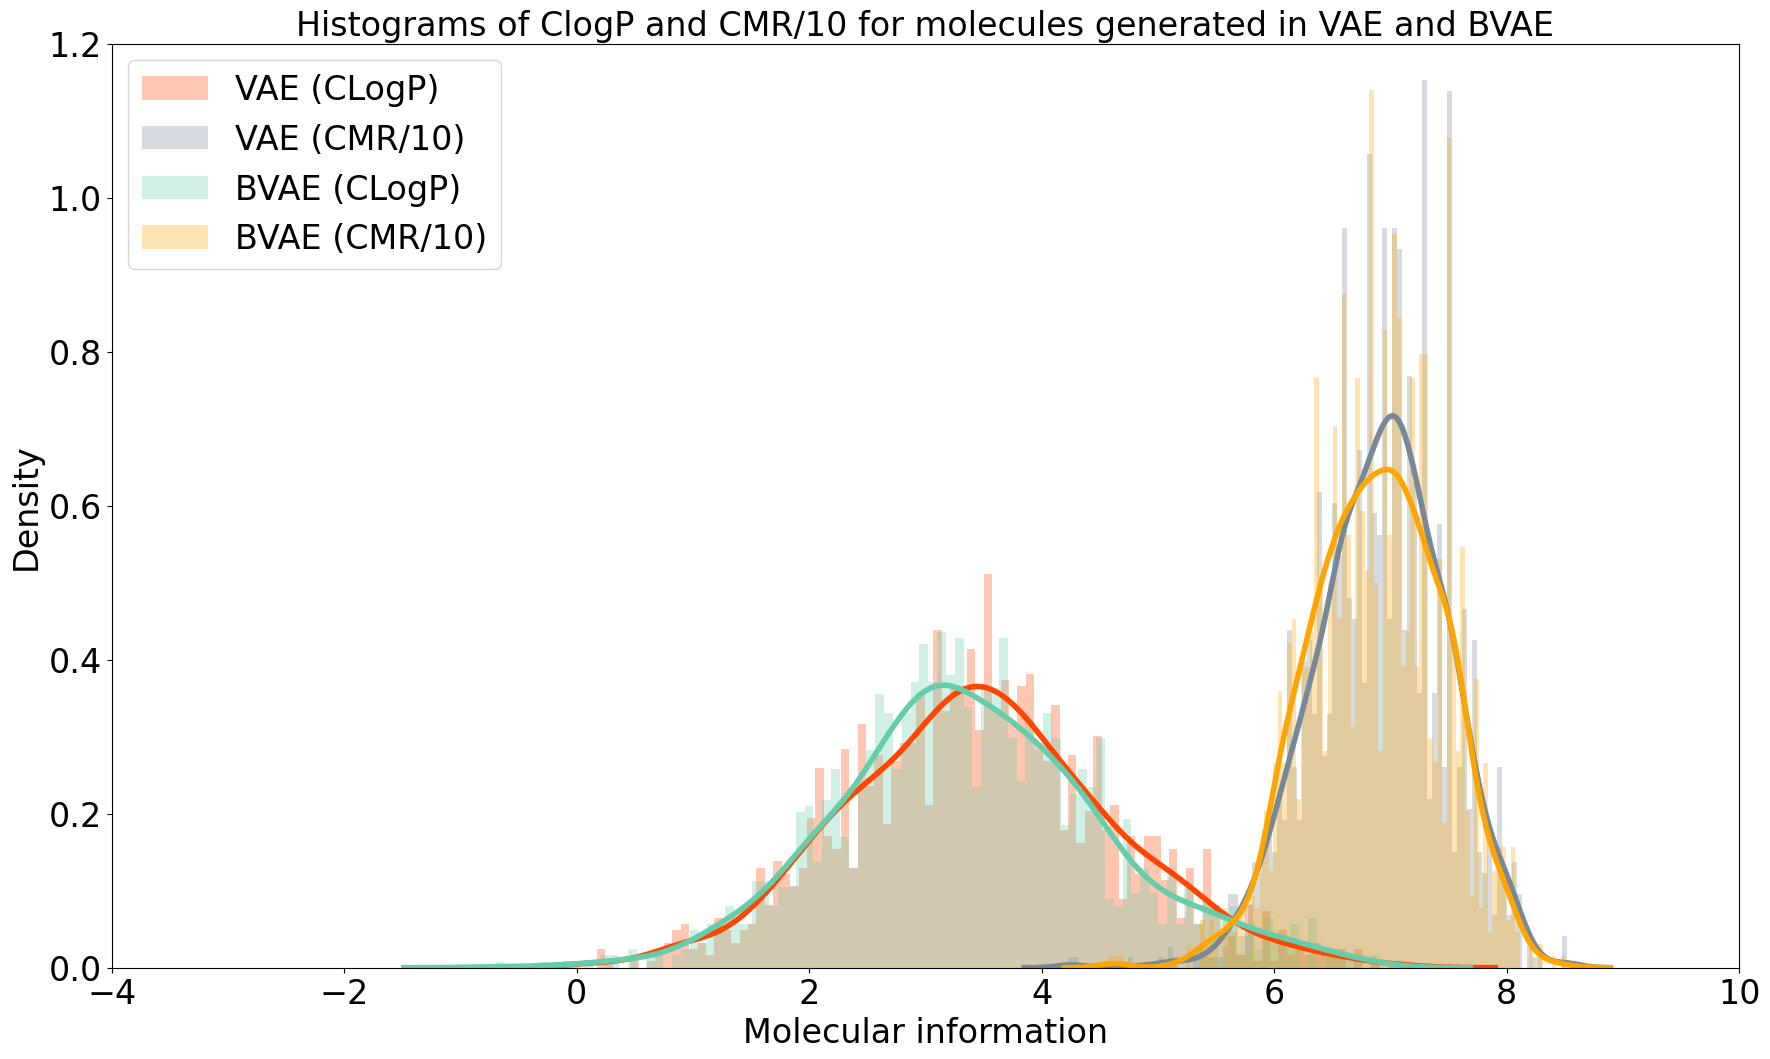
\includegraphics[width=0.7\textwidth]{fig6.png}}
    \caption{Histograms of the molecular information generated by VAE and $\beta$-VAE.}
    \label{fig}
\end{figure}

With reference to Table 3, it can be observed that the mean values of ClogP and CMR of generated molecules decrease in order of VAE, $\beta$-VAE, CVAE, and $\beta$-CVAE. This suggests that more complex models aim to generate molecules with properties similar to that of the data set ClogP $= 0.929$ and CMR $= 63.063$. Moreover, the proposed $\beta$-CVAE model generated the most molecules with properties closer to the data set. This result complements the results from \cite{meyers2021novo, richards2022conditional}, which suggests that the disentanglement factor and conditional vector improve the molecular property optimization results. 

\section{Multi-objective optimization}
Thus far, we examined the single-property optimization results. Now, let us have a look at the multi-objective (two-property) optimization results with respect to the conditional requirements in (6). With reference to Table 4, our model produced the best results for both single-objective optimizations ("ClogP (\%)" and "CMR (\%)") and multi-objective optimization ("Both (\%)"). The best pairwise target properties within the range of $C1 \pm 0.5$ and $C2 \pm 5$ are $C1 = 2$ and  $C2 = 70$. Our model generated 33.351\% of molecules within the desired condition of ClogP $= 2$. Similarly, 74.871\% of generated molecules were within the desired condition of CMR $= 70$. Moreover, our model generated 26.680\% of molecules that satisfies both target properties. In comparison to results in \cite{lee2022mgcvae}, our proposed molecular graph $\beta$-CVAE generated a higher percentage of molecules that satisfies both properties. 

Comparing our model to the other models, the $\beta$-CVAE performed slightly poorer than the CVAE in multi-objective optimization when C1 $= 3$. Turning our attention to the C1$ = 4$ and C1 $= 5$, the VAE model outperforms its advanced counterparts. Despite our model producing the best results for the CMR property, the VAE generated the best multi-objective optimization results of 22.882\% and 7.353\% for C1$ = 4$ and C1 $= 5$, respectively.

\begin{table*}[t]
\caption{Condition results}
\centering
\resizebox{\textwidth}{!}{%
\begin{tabular}{|ccccc|ccccc|ccccc|ccccc|}
\hline
\multicolumn{5}{|c|}{VAE} & \multicolumn{5}{c|}{$\beta$-VAE} & \multicolumn{5}{c|}{CVAE} & \multicolumn{5}{c|}{\textbf{$\beta$-CVAE}} \\ \hline
\textbf{CLogP (\%)} & \textbf{CMR (\%)} & \textbf{Both (\%)} & \textbf{C1} & \textbf{C2} & \textbf{CLogP (\%)} & \textbf{CMR (\%)} & \textbf{Both (\%)} & \textbf{C1} & \textbf{C2} & \textbf{CLogP (\%)} & \textbf{CMR (\%)} & \textbf{Both (\%)} & \textbf{C1} & \textbf{C2} & \textbf{CLogP (\%)} & \textbf{CMR (\%)} & \textbf{Both (\%)} & \textbf{C1} & \textbf{C2} \\ \hline
0.471 & 0.000 & 0.000 & 0 & 20 & 0.613 & 0.000 & 0.000 & 0 & 20 & 4.016 & 0.000 & 0.000 & 0 & 20 & \textbf{10.196} & 0.000 & 0.000 & 0 & 20 \\
0.471 & 0.000 & 0.000 & 0 & 30 & 0.613 & 0.000 & 0.000 & 0 & 30 & 9.739 & 0.000 & 0.000 & 0 & 30 & \textbf{32.456} & \textbf{11.842} & \textbf{4.386} & 0 & 30 \\
0.471 & 0.118 & 0.000 & 0 & 40 & 0.613 & 0.000 & 0.000 & 0 & 40 & 4.628 & 1.983 & 0.000 & 0 & 40 & \textbf{22.878} & \textbf{6.089} & \textbf{1.107} & 0 & 40 \\
0.471 & 0.647 & 0.118 & 0 & 50 & 0.613 & 1.043 & 0.184 & 0 & 50 & 4.887 & 18.935 & 2.705 & 0 & 50 & \textbf{13.357} & \textbf{29.371} & \textbf{7.133} & 0 & 50 \\
0.471 & 20.765 & 0.294 & 0 & 60 & 0.613 & 24.417 & 0.429 & 0 & 60 & 1.508 & 36.704 & 1.117 & 0 & 60 & \textbf{5.838} & \textbf{55.288} & \textbf{4.738} & 0 & 60 \\
0.471 & 63.000 & 0.059 & 0 & 70 & 0.613 & 59.448 & 0.000 & 0 & 70 & 0.219 & 64.262 & 0.164 & 0 & 70 & \textbf{3.42} & \textbf{79.654} & \textbf{2.035} & 0 & 70 \\ \hline
3.235 & 0.000 & 0.000 & 1 & 20 & 3.558 & 0.000 & 0.000 & 1 & 20 & 15.127 & 0.000 & 0.000 & 1 & 20 & \textbf{25.824} & 0.000 & 0.000 & 1 & 20 \\
3.235 & 0.000 & 0.000 & 1 & 30 & 3.558 & 0.000 & 0.000 & 1 & 30 & 30.187 & 0.187 & 0.000 & 1 & 30 & \textbf{30.422} & \textbf{23.795} & \textbf{7.831} & 1 & 30 \\
3.235 & 0.118 & 0.000 & 1 & 40 & 3.558 & 0.000 & 0.000 & 1 & 40 & 22.687 & 5.286 & 3.084 & 1 & 40 & \textbf{32.329} & \textbf{12.055} & \textbf{4.658} & 1 & 40 \\
3.235 & 0.647 & 0.176 & 1 & 50 & 3.558 & 1.043 & 0.245 & 1 & 50 & 20.925 & 33.754 & 10.305 & 1 & 50 & \textbf{30.757} & \textbf{42.962} & \textbf{17.087} & 1 & 50 \\
3.235 & 20.765 & 2.412 & 1 & 60 & 3.558 & 24.417 & 2.331 & 1 & 60 & 8.265 & 41.199 & 6.751 & 1 & 60 & \textbf{19.917} & \textbf{55.602} & \textbf{15.952} & 1 & 60 \\
3.235 & 63.000 & 0.647 & 1 & 70 & 3.558 & 59.448 & 0.982 & 1 & 70 & 3.398 & 69.127 & 2.46 & 1 & 70 & \textbf{15.106} & \textbf{77.732} & \textbf{9.963} & 1 & 70 \\ \hline
16.647 & 0.000 & 0.000 & 2 & 20 & 15.951 & 0.000 & 0.000 & 2 & 20 & 34.176 & 0.000 & 0.000 & 2 & 20 & \textbf{37.280} & 0.000 & 0.000 & 2 & 20 \\
16.647 & 0.000 & 0.000 & 2 & 30 & 15.951 & 0.000 & 0.000 & 2 & 30 & \textbf{43.363} & 0.442 & 0.221 & 2 & 30 & 18.487 & \textbf{21.008} & \textbf{1.120} & 2 & 30 \\
16.647 & 0.118 & 0.059 & 2 & 40 & 15.951 & 0.000 & 0.000 & 2 & 40 & \textbf{42.663} & 6.250 & 1.630 & 2 & 40 & 29.944 & \textbf{14.972} & \textbf{4.802} & 2 & 40 \\
16.647 & 0.647 & 0.294 & 2 & 50 & 15.951 & 1.043 & 0.368 & 2 & 50 & 35.601 & 41.950 & \textbf{18.141} & 2 & 50 & \textbf{36.015} & \textbf{49.298} & 16.838 & 2 & 50 \\
16.647 & 20.765 & 8.059 & 2 & 60 & 15.951 & 24.417 & 8.466 & 2 & 60 & 23.507 & 41.106 & 15.713 & 2 & 60 & \textbf{35.801} & \textbf{57.910} & \textbf{24.432} & 2 & 60 \\
16.647 & 63.000 & 8.176 & 2 & 70 & 15.951 & 59.448 & 7.055 & 2 & 70 & 17.430 & 71.374 & 13.295 & 2 & 70 & \textbf{33.351} & \textbf{74.871} & \textbf{26.680} & 2 & 70 \\ \hline
31.118 & 0.000 & 0.000 & 3 & 20 & \textbf{34.724} & 0.000 & 0.000 & 3 & 20 & 33.770 & 0.000 & 0.000 & 3 & 20 & 13.936 & 0.000 & 0.000 & 3 & 20 \\
31.118 & 0.000 & 0.000 & 3 & 30 & \textbf{34.724} & 0.000 & 0.000 & 3 & 30 & 21.076 & 0.110 & 0.000 & 3 & 30 & 9.048 & \textbf{16.190} & \textbf{0.952} & 3 & 30 \\
31.118 & 0.118 & 0.059 & 3 & 40 & \textbf{34.724} & 0.000 & 0.000 & 3 & 40 & 26.415 & \textbf{4.852} & \textbf{0.539} & 3 & 40 & 15.625 & 2.083 & 0.000 & 3 & 40 \\
31.118 & 0.647 & 0.059 & 3 & 50 & \textbf{34.724} & 1.043 & 0.184 & 3 & 50 & 31.179 & \textbf{42.839} & \textbf{10.646} & 3 & 50 & 16.406 & 28.516 & 2.734 & 3 & 50 \\
31.118 & 20.765 & 7.706 & 3 & 60 & 34.724 & 24.417 & \textbf{10.429} & 3 & 60 & \textbf{36.926} & 42.743 & 16.289 & 3 & 60 & 17.088 & \textbf{54.392} & 6.378 & 3 & 60 \\
31.118 & 63.0 & 22.765 & 3 & 70 & 34.724 & 59.448 & 22.761 & 3 & 70 & \textbf{35.229} & 71.359 & \textbf{31.623} & 3 & 70 & 25.526 & \textbf{74.174} & 22.222 & 3 & 70 \\ \hline
\textbf{30.706} & 0.000 & 0.000 & 4 & 20 & 29.325 & 0.000 & 0.000 & 4 & 20 & 4.124 & 0.000 & 0.000 & 4 & 20 & 3.768 & 0.000 & 0.000 & 4 & 20 \\
\textbf{30.706} & 0.000 & 0.000 & 4 & 30 & 29.325 & 0.000 & 0.000 & 4 & 30 & 0.452 & 0.754 & 0.000 & 4 & 30 & 0.000 & \textbf{23.188} & 0.000 & 4 & 30 \\
\textbf{30.706} & 0.118 & 0.000 & 4 & 40 & 29.325 & 0.000 & 0.000 & 4 & 40 & 1.337 & 8.556 & 0.000 & 4 & 40 & 1.201 & \textbf{11.712} & 0.000 & 4 & 40 \\
\textbf{30.706} & 0.647 & 0.000 & 4 & 50 & 29.325 & 1.043 & 0.000 & 4 & 50 & 6.757 & 48.025 & \textbf{1.767} & 4 & 50 & 2.836 & \textbf{51.996} & 0.735 & 4 & 50 \\
\textbf{30.706} & 20.765 & 2.176 & 4 & 60 & 29.325 & 24.417 & 2.331 & 4 & 60 & 13.162 & 53.276 & \textbf{3.476} & 4 & 60 & 7.117 & \textbf{62.058} & 1.126 & 4 & 60 \\
\textbf{30.706} & 63.0 & \textbf{22.882} & 4 & 70 & 29.325 & 59.448 & 21.288 & 4 & 70 & 26.075 & 71.748 & 16.918 & 4 & 70 & 14.07 & \textbf{77.722} & 9.994 & 4 & 70 \\ \hline
\textbf{13.647} & 0.000 & 0.000 & 5 & 20 & 10.798 & 0.000 & 0.000 & 5 & 20 & 0.285 & 0.000 & 0.000 & 5 & 20 & 0.375 & 0.000 & 0.000 & 5 & 20 \\
\textbf{13.647} & 0.000 & 0.000 & 5 & 30 & 10.798 & 0.000 & 0.000 & 5 & 30 & 0.000 & 1.173 & 0.000 & 5 & 30 & 0.000 & \textbf{22.941} & 0.000 & 5 & 30 \\
\textbf{13.647} & 0.118 & 0.000 & 5 & 40 & 10.798 & 0.000 & 0.000 & 5 & 40 & 0.000 & 9.296 & 0.000 & 5 & 40 & 0.000 & \textbf{11.709} & 0.000 & 5 & 40 \\
\textbf{13.647} & 0.647 & 0.000 & 5 & 50 & 10.798 & 1.043 & 0.0 & 5 & 50 & 1.204 & 48.546 & \textbf{0.502} & 5 & 50 & 0.201 & \textbf{55.065} & 0.000 & 5 & 50 \\
\textbf{13.647} & 20.765 & 0.118 & 5 & 60 & 10.798 & 24.417 & \textbf{0.429} & 5 & 60 & 4.096 & 51.65 & 0.284 & 5 & 60 & 0.984 & \textbf{61.192} & 0.207 & 5 & 60 \\
\textbf{13.647} & 63.0 & \textbf{7.353} & 5 & 70 & 10.798 & 59.448 & 6.258 & 5 & 70 & 9.38 & 71.511 & 3.59 & 5 & 70 & 3.413 & \textbf{76.869} & 1.463 & 5 & 70 \\ \hline
\end{tabular}%
}
\end{table*}

\begin{figure*}
    \centering
    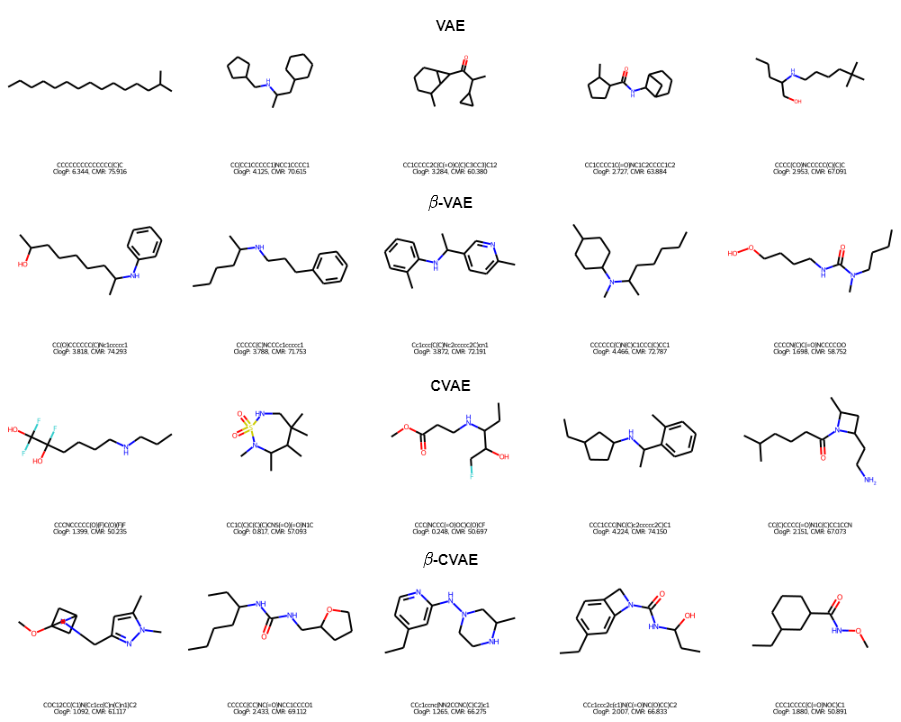
\includegraphics[width=1\textwidth]{fig5.png}
    \caption{Sample of generated molecules from VAE, $\beta$-VAE, CVAE, and $\beta$-CVAE models, respectively.}
    \label{fig:img1}
\end{figure*}
